\documentclass[UTF8, 12pt]{article}
\usepackage{xeCJK}
\usepackage{ctex}
\usepackage{amsmath,amssymb,amsthm,amsfonts,amscd}
\usepackage{fontspec}
\setmainfont{Times New Roman}
\usepackage{graphicx}
\usepackage{titlesec}
\usepackage{makecell}
\usepackage{longtable}
\usepackage{xcolor}
\usepackage{tcolorbox}
\usepackage{soul}
\usepackage{adjustbox}
\usepackage{tcolorbox}
\usepackage{enumerate}
\usepackage{pdfpages}
\usepackage{float}
\usepackage{colortbl}
\usepackage{tabularx}
\usepackage{multirow}
\usepackage{pgfplots}
\numberwithin{figure}{section}
\usepackage[left=1.25in,right=1.25in,%
top=1in,bottom=1in]{geometry}
\usepackage{color}
\usepackage{pifont}       % \ding{xx}
\usepackage{bbding}
\usepackage{subfigure}
\titleformat{\section}
  {\center\LARGE\bfseries}{\thesection}{1em}{}

  \newcommand{\upcite}[1]{$^{\scriptsize \cite{#1}}$}
  \newcommand{\crossmark}{\ding{55}}
\linespread{1.5}

\begin{document}
\title{\heiti 文章《Spatial Deep Learning for Wireless Scheduling》的解读}
\date{}
\maketitle
\begin{center}
    \heiti \large 摘要
\end{center}

在一个充分频率复用的密集无线网络中,对相互干扰链路的优化调度是一项具有挑战性的任务。传统方法首先估算所有干扰通道的强度,然后基于模型优化调度。然而,这种基于模型的方法对资源的消耗大,计算量也大,因为在密集网络中估算通道的消耗大;而且,找到由此产生的优化问题的局部最优解可能在计算上复杂。本文表明,通过使用深度学习方法,可以绕过通道估算,并仅基于发射机和接收机的地理位置高效地调度链路,这是因为在许多传播环境中,无线通道的强度大部分是距离依赖性路径损耗的函数。这是通过在随机部署的网络上进行无监督训练,通过使用一种新颖的神经网络架构,该架构计算了与干扰或被干扰的相邻节点的地理空间卷积以及后续多阶段反馈,以学习最优解。得到的神经网络为总速率最大化提供了接近最优的性能,并且能够推广到更大的部署区域和不同的链路密度部署。此外,为了提供公平性,本文提出了一种新颖的调度方法,该方法利用总速率最优调度算法,在巧妙选择的子链路集上,以最大化网络的比例公平目标。所提出的方法展示了具有高度竞争力和可泛化的网络效用最大化结果。

\vspace{1em}

\heiti \textbf{关键词:} 无线网络,深度学习,调度,空间卷积,链路优化
\clearpage

\section{文章主要内容}
\subsection{引言}
\songti 在无线网络中,干扰链路的调度是一项基础且关键的任务。考虑一个高密度部署的设备对设备(D2D)网络,这里采用全频率复用,相邻链路在同时激活时会对彼此产生显著干扰。调度的任务是明智地激活一组相互“兼容”的链路子集,以避免过度干扰,从而最大化网络效用。传统的链路调度方法基于首先估计干扰信道的范式,但这种方法在资源和计算上都相当密集(或至少干扰图拓扑结构的估计),然后基于估计的信道来优化调度。然而,这种基于模型的方法有两个主要缺点。首先,不仅需要估计直接信道,还需要估计所有的干扰信道,这是非常消耗资源的。在一个由N个发射接收对组成的网络中,每个相干块内需要估计$N^2$个信道。训练会从实际数据传输中占用宝贵的资源;此外,在大型网络中,导频污染是不可避免的。其次,干扰环境中的实现数据率是发射功率的非凸函数。更重要的是,调度变量是二进制的。因此,即使在完全知道信道的情况下,调度优化也是一个非凸整数规划问题,找到最优解在计算上是复杂的,对于实时实施来说是具有挑战性的。

本文提出了一种新的方法,名为空间深度学习,来解决上述两个问题。作者的核心思想是认识到在很多部署场景中,最优链路调度并不一定需要精确的信道估计,而且网络中的干扰模式在很大程度上由发射机和接收机的相对位置决定。因此,作者应该可以仅根据邻近发射机/接收机的地理位置来学习最优调度,从而完全绕过信道估计。为此,本文提出了一种神经网络架构,该架构计算出干扰或受干扰的邻近发射机/接收机位置的地理空间卷积,并在基于空间参数的多个反馈阶段内,学习在密集部署的D2D网络中的最优调度。

作者受到了最近机器学习技术成功应用剧增的启发,这些应用证明了深度神经网络具有学习丰富模式和近似任意函数映射的能力。作者进一步利用了最近在链路调度的分数规划方法上取得的进展,这使作者能够与最先进的基准进行比较。本文的主要贡献之一是设计了一个专门的神经网络架构,它促进了对干扰或受干扰节点的地理位置进行空间学习,并且在计算上能以高效的方式达到最先进算法的最大吞吐率的大部分,同时不需要明确的信道状态信息。

\subsection{研究现状}

在传统的无线干扰链路调度方法中,为了实现总速率最大化,通常基于非凸优化策略,例如贪心启发式搜索\upcite{FlashLinQ}、迭代方法以达成高质量局部最优\upcite{shen_ISIT17, luo_TSP11}、基于信息理论考虑的方法\upcite{ITLinQ,ITLinQ+}或超图着色\upcite{Guo_TCOM17,color},以及实现全局最优但面临最坏情况指数级复杂性的方法,如基于多面体块的优化\upcite{MAPEL}或非线性列生成\upcite{Johansson_TWC06}。近期,机器学习的复兴促进了神经网络在无线网络优化中的应用。本研究与\upcite{hong_spawc, alejandro}的最新工作密切相关,这些工作将深度学习应用于功率控制,以及\upcite{cong_ensemble}利用集成学习解决相关问题。与\upcite{hong_spawc, cong_ensemble, alejandro}的研究相比,作者进一步创新,放弃了频谱优化中的传统信道状态信息(CSI)要求。本文证明,在信道增益主要由路径损耗决定的无线网络中,位置信息(通过全球定位系统容易获取)可以有效地作为近似最优解的代理,为学习理论在无线网络资源分配问题中的更广泛应用开启新的可能性。

\subsection{问题背景}

考虑一个位于二维区域内的$N$个独立D2D链路的场景。链路之间的发射机-接收机距离是可变的。作者使用$p_i$来表示第$i$个链路的固定传输功率水平,如果它被激活的话。此外,作者用$h_{ij}\in\mathbb C$来表示第$j$个链路的发射机到第$i$个链路的接收机的信道,并用$\sigma^2$表示背景噪声功率水平。调度是以时间槽方式进行的。在每个时间槽中,让$x_i\in{0,1}$表示每个链路$i$的指示变量,当链路被调度时,其值为1,否则为0。作者假设频宽$W$下的全频率复用。给定一组调度决策$x_i$,链路$i$在时间槽中的可达速率$R_i$可以计算为

\begin{align}
R_i =W\log\left(1+\frac{|h_{ii}|^2p_ix_i}{\Gamma(\sum_{j\neq i}|h_{ij}|^2 p_jx_j + \sigma^2)}\right),
\end{align}

其中$\Gamma$是信噪比(SNR)与信息理论信道容量之间的差距,这是由于在线性高斯信道中使用实际的编码和调制所致 \upcite{forney}。由于链路之间的相互干扰,同时激活所有链路会导致数据速率降低。无线链路调度问题是选择在任何给定的传输周期内激活的链路子集,以最大化实现的速率的网络效用函数。

本文考虑的目标函数是在每个调度时隙内最大化$N$个用户的加权和速率。更具体地说,对于固定的权重值$w_i$,调度问题被表述为

\begin{subequations}
  \label{prob}
  \begin{align}
  \underset{\mathbf{x}}{\text{maximize}}\quad&
  \sum^N_{i=1} w_i R_i\\
  \text{subject to}\quad& x_i \in \{0,1\},\;\forall i.
  \end{align}
  \end{subequations}

权重$w_i$表示分配给每个用户的优先级(即,优先级更高的用户更有可能被调度)。整个问题是一个挑战性的离散优化问题,这是由于不同链路通过信号干扰和噪声(SINR)表达式中的干扰项相互作用,以及每个用户可能具有的不同优先级权重。

\begin{align}
\max \sum_{i=1}^N w_i R_i
\end{align}

其中$R_i$是链路$i$在当前时间槽内的可达速率,如上所述。这个问题的挑战在于,链路之间的相互干扰和功率限制,使得不可能同时激活所有链路。因此,必须制定一个有效的调度策略,以在给定的网络条件下实现最佳的总体性能。

\clearpage 

\subsection{问题分析}

本文首先探讨在总速率最大化准则下,仅利用位置信息使用深度神经网络进行调度的方法。总速率最大化问题(即,等权重)比加权速率和最大化简单得多,因为所有链路具有相同的优先级。本文的目标是使用路径损耗和地理位置信息来确定应该调度哪些链路子集。

  \subsubsection{基于地理位置信息的学习}

  本文的一个核心目标是展示,在无线网络中,如果信道增益主要是距离相关的路径损耗函数,那么地理位置信息就足以作为优化链路调度的代理。这与传统的优化方法形成对比,传统方法需要完整的即时信道状态信息(CSI)来解决问题 (\ref{prob}),也与最近的研究工作\cite{hong_spawc}形成对比,该研究提议使用深度学习来解决功率控制问题,通过学习WMMSE优化过程。在\cite{hong_spawc}中,设计了一个全连接的神经网络,它以信道系数矩阵为输入,产生优化的连续功率变量作为输出,以最大化总速率。虽然在\cite{hong_spawc}中获得了令人满意的调度性能,但\cite{hong_spawc}的架构不具可扩展性。在一个有$N$个发射机-接收机对的D2D链路网络中,有$N^2$个信道系数。一个在输入层有$N^2$个节点,在输出层有$N$个节点的全连接神经网络至少需要$O(N^3)$的互连权重(而且很可能更多)。因此,\cite{hong_spawc}提出的神经网络架构的训练和测试复杂性随着链路数量的增加而迅速增长。
  
  作者提议的不是需要每个发射机和每个接收机之间的完整CSI集作为神经网络的输入${h_{ij}}$,这需要$O(N^2)$个条目,而是提议使用地理位置信息(GLI)作为输入,定义为一组向量${(\mathbf d^{\text{tx}}{i},\mathbf d^{\text{rx}}{i})}i$,其中$\mathbf d^{\text{tx}}{i}\in\mathbb R^2$和$\mathbf d^{\text{rx}}_{i}\in\mathbb R^2$分别是第$i$个链路的发射机和接收机位置。注意,输入现在与链路数量线性相关,即$O(N)$。
  
  作者主张使用GLI作为CSI的替代品,因为在许多无线部署场景中,GLI已经捕捉到了信道的主要特征:无线链路的路径损耗和阴影效应主要是距离和位置的函数。这对于户外无线信道尤其如此,特别是在农村地区或偏远地区,周围反射无线信号的物体数量稀少。一个例子是部署在户外进行环境监测的传感器网络。
  
  事实上,如果还考虑到快速衰落,那么CSI可以被认为是GLI的随机函数

  \begin{equation}
  \text{CSI} = f(\text{GLI}).
  \end{equation}

  虽然无线链路调度问题的优化方法旨在找到从CSI到调度决策的映射$g(\cdot)$,即

  \begin{equation}
  \mathbf x = g(\text{CSI}),
  \end{equation}

  但本文的深度学习架构旨在直接捕捉从GLI到$\mathbf x$的映射,即学习函数
  
  \begin{equation}
  \mathbf x = g(f(\text{GLI})).
  \end{equation}



\subsection{作为输入的发射机和接收机密度网格}

为了基于GLI构建神经网络的输入,作者将连续的$(\mathbf d^{\text{tx}}{i}, \mathbf d^{\text{rx}}{i})$量化为网格形式。不失一般性,作者假设一个$\ell \times \ell$米的部署区域,划分为边长为$\ell/M$的等大小正方形单元格,总共有$M^2$个单元格。作者使用$(s,t)\in[1:M]\times[1:M]$来索引单元格。对于特定的链路$i$,让$(s^\text{tx}_i,t^\text{tx}_i)$是发射机$\mathbf d^\text{tx}_i$所在单元格的索引,$(s^\text{rx}_i,t^\text{rx}_i)$是接收机$\mathbf d^\text{rx}_i$所在单元格的索引。作者使用元组$(s^\text{tx}_i,t^\text{tx}_i,s^\text{rx}_i,t^\text{rx}_i)$来表示链路的位置信息。

作者提议构建两个大小为$M \times M$的\emph{密度网格}矩阵,分别用$T$和$R$表示,来代表地理区域内\emph{活动}发射机和接收机的密度。密度网格矩阵通过简单地计算每个单元格中活动发射机和接收机的总数来构建,如图~\ref{fig:gridexplain}所示。激活模式${ x_i }$最初被初始化为全1向量。随着算法逐步更新激活模式,密度网格矩阵也随之更新
\begin{eqnarray}
  \label{eq:grid_tx}
  T(s,t) & = & \sum_{\{i | (s^\text{tx}_i,t^\text{tx}_i) = (s,t) \}} x_i, \\
  R(s,t) & = & \sum_{\{i | (s^\text{rx}_i,t^\text{rx}_i) = (s,t) \}} x_i.
  \label{eq:grid_rx}
  \end{eqnarray}
  
  \clearpage

  \begin{figure*}[htbp]
    \centering
    \centerline{\includegraphics[width=13cm]{fig/GridExplain}}
    \caption{发射机和接收机密度网格}
    \label{fig:gridexplain}
    \end{figure*}


\subsubsection{神经网络结构 }

针对总速率目标的链路调度的整体神经网络结构是一个迭代计算图。网络结构的一个关键新特性是包含两个阶段的前向路径:一个卷积阶段,基于地理位置信息捕获邻近链路的干扰模式;一个全连接阶段,捕获优化调度的非线性功能映射。此外,作者提出了一个新颖的\emph{反馈连接},用于更新优化状态。以下详细描述了各个阶段和整体网络结构。
\begin{figure}[htbp]
  \centering
  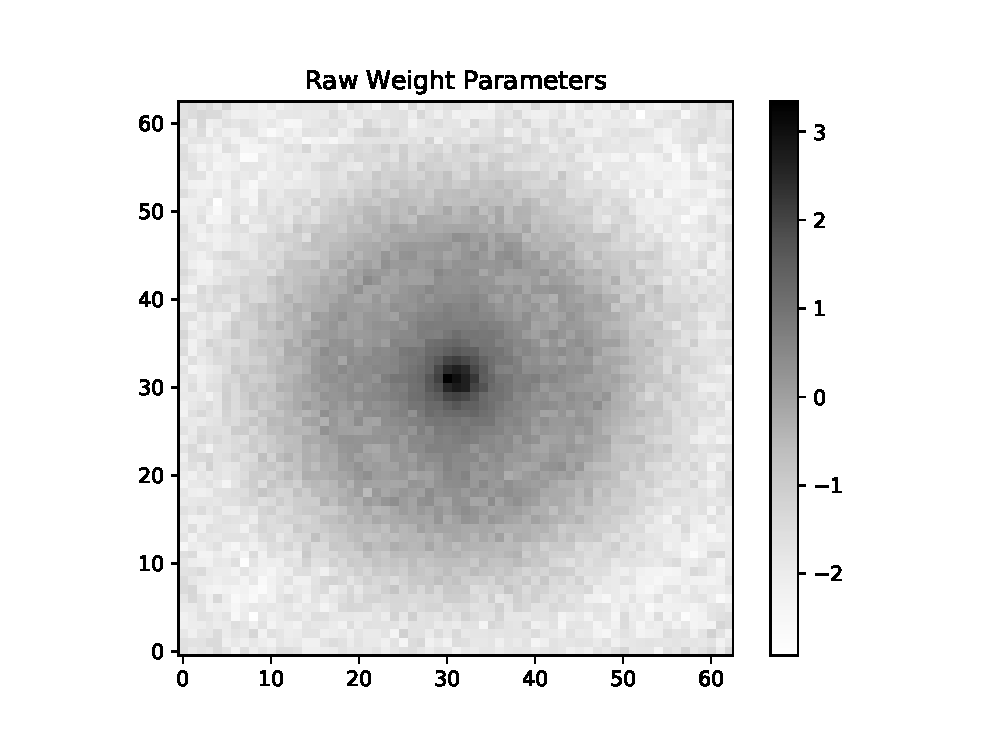
\includegraphics[width=7.5cm]{fig/ConvFilter}
  \caption{训练后的空间卷积滤波器(对数尺度)}
  \label{fig:convfilter}
  \end{figure}
  
\begin{enumerate}

  \item \textbf{卷积阶段}
  
  卷积阶段负责计算两个函数,分别对应于每个链路对其邻居造成的干扰和每个链路从其邻居处接收的干扰。作为神经网络架构的主要创新,作者提出使用空间卷积滤波器,其系数在训练过程中进行优化,直接作用于前一节中描述的发射机和接收机密度网格。发射机和接收机的空间卷积在两个网格上并行计算。最后,为每个链路的发射机-接收机对计算出两个信息:一个是发射机\emph{可能对其造成干扰的}所有附近接收机的空间地理位置的卷积;另一个是接收机\emph{可能从其经历干扰的}所有附近发射机的空间地理位置的卷积。这些计算出的卷积分别称为链路$i$的TxINT$_i$和RxINT$_i$。
  
  卷积滤波器是一个具有固定预定义大小和可训练参数的2D正方形矩阵。滤波器中每个条目的值可以解释为位于滤波器中心一定距离处的收发器的信道系数。通过训练,滤波器通过调整其权重来学习信道系数。图~\ref{fig:convfilter}显示了一个训练后的滤波器。正如预期的那样,训练后的滤波器显示出具有径向衰减的圆形对称模式。
  
  上述卷积阶段为每个链路总结了两个量:发射机产生的总干扰和接收机暴露于的总干扰。此外,作者表示还可以从训练后的卷积滤波器中提取另一个重要的调度量:\emph{直接信道强度}。在发射机相对于其接收机的相应相对位置,卷积滤波器的值描述了这对发射机/接收机之间直接链路的信道增益。获取此直接信道强度的过程在图~\ref{fig:directchannelstrength}中进行了说明。链路$i$的直接信道强度被称为DCS$_i$。
  
  \begin{figure}
  \centering
  \includegraphics[width=12cm]{fig/DirectChannelStrength}
  \caption{从卷积滤波器提取直接信道强度}
  \label{fig:directchannelstrength}
  \end{figure}
  
  \item \textbf{全连接阶段}
  
  全连接阶段是前向计算路径的第二阶段,紧接在上述卷积阶段之后。它以为每个链路提取的特征向量为输入,并为该链路产生一个输出$x_i \in [0,1]$(可以解释为松弛调度变量或替代为连续功率)。

\begin{figure*}
\centering
\centerline{\includegraphics[width=13cm]{fig/ForwardPath}}
\caption{单个链路的前向计算路径,其中包括空间卷积和链路距离作为神经网络的输入}
\label{fig:fpath}
\end{figure*}

每个链路的特征向量包括以下条目:TxINT$i$、RxINT$i$、DCS$i$、DCS${\max}$、DCS${\min}$、$x{i}^{t-1}$。前三个术语已在前一节中解释。DCS${\max}$和DCS${\min}$分别表示整个布局中链路直接信道强度的最大值和最小值;$x_{i}^{t-1}$表示整体反馈结构中前一次迭代的全连接阶段输出。元组(TxINT$_i$、RxINT$i$)描述了第$i$个链路与其邻居之间的干扰,而三元组(DCS$i$、DCS${\max}$、DCS${\min}$)描述了与整个布局中最强和最弱链路相比的链路自身的信道强度。

链路的值$x_i$是基于其特征向量通过全连接神经网络(这里表示为$F_{fc}$)的功能映射计算的,这在反馈迭代中由$t$索引:

\begin{align}
x_{i}^{t} \gets F_{fc}(\text{TxINT}{i}, \text{RxINT}{i}, \text{DCS}{i}, \text{DCS}{\max}, \text{DCS}{\min}, x{i}^{t-1}).
\end{align} 

卷积阶段和全连接阶段共同构成了每对发射机-接收机的一个前向计算路径,如图~\ref{fig:fpath}所示。在实现中,作者使用了两个隐藏层,每层有30个神经元,以确保神经网络的足够表达能力。在隐藏层的每个神经元中使用了修正线性单元(ReLU);在输出节点使用了Sigmoid非线性函数,以产生一个位于$[0,1]$范围内的值。

\item \textbf{反馈连接}\label{sec:feedbacksection}

前向计算(包括卷积阶段和全连接阶段)将链路激活模式$x_i$作为输入,用于构建密度网格。为了考虑通过迭代过程中无线链路的逐步(解)激活模式(即,每个后续的干扰估计都需要意识到被解激活的链路不再产生或受到干扰),作者提出了一个反馈结构。在这个结构中,神经网络的每次迭代都将上一次迭代的连续输出$x$作为输入,然后进行固定次数的迭代。作者通过实验发现,网络能够在少量迭代内收敛。

反馈阶段的设计如下:在完成第$(t-1)$次前向计算后,获得了代表$N$个链路激活状态的$[0,1]$值的$\mathbf x$向量。然后,通过将这个$\mathbf x$向量输入到(\ref{eq:grid_tx})-(\ref{eq:grid_rx})中,开始新的前向计算,并准备输入密度网格。通过这种方式,所有$N$个链路的激活状态在密度网格中得到更新,用于后续的干扰估计。

需要注意的是,卷积滤波器和神经网络的可训练权重在多次迭代中是绑定在一起的,以便于更有效的训练。

\begin{figure*}[htbp]
\centering
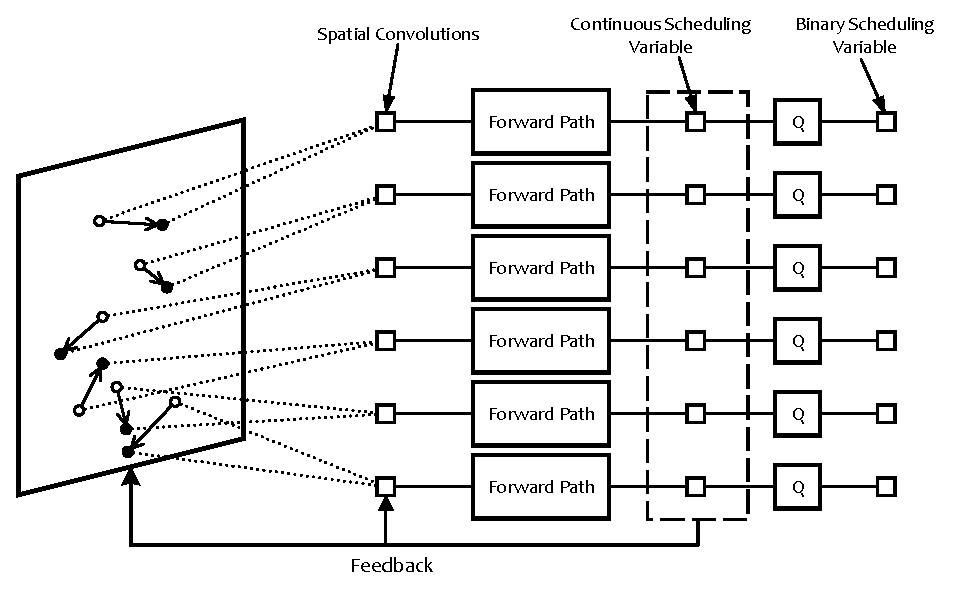
\includegraphics[width=12cm]{fig/learning_model}
\caption{整体神经网络,每个链路有一个前向路径,带有反馈连接和量化输出(标记为“Q”)。}
\label{fig:feedback}
\end{figure*}

在固定数量的迭代后,通过将最后一次迭代中的$\mathbf x$向量量化为二进制值来获取神经网络的调度决策,这些二进制值代表$N$个链路的调度决策。

整体反馈结构如图~\ref{fig:feedback}所示。作者在这里强调,神经网络是基于每个链路设计的,因此整体模型可以根据网络规模进行扩展。具体来说,在卷积阶段,根据固定(并经过训练)的卷积滤波器计算卷积,该滤波器覆盖了邻近的不可忽视的干扰源。在全连接阶段,不同链路的神经网络是解耦的,因此调度可以以分布式方式进行。

此外,在训练阶段,不同链路的卷积滤波器参数和神经网络权重是绑定在一起的。这有助于高效的训练,并隐含地假设不同链路的传播环境是相似的。在这种同质性假设下,无论布局有多大,网络中需要调度多少链路,整个训练后的神经网络模型都可以直接用于调度,无需调整或重新训练。
\end{enumerate}

\subsection{训练和测试}

考虑到篇幅限制,这里仅说明对于与训练样本大小相同的布局上的测试和引入快衰落的测试。
\subsubsection{训练流程}

作者随机生成了由$N=50$对D2D链路组成的无线D2D网络,这些网络位于500米乘500米的区域内。发射机的位置在该区域内均匀生成。接收机的位置根据从它们各自的发射机相距$d_{\min}\sim d_{\max}$米的均匀分布生成。作者为训练生成了800,000个这样的网络布局。

发射机-接收机距离对可达速率有显著影响。为总速率最大化进行链路调度倾向于优先考虑短链路而非长链路,因此链路距离的分布对调度性能有显著影响。为了发展所提出的深度学习方法适应不同的发射机-接收机距离,作者根据以下分布生成训练样本:

\begin{itemize}
\item 从$2\sim70$米中均匀生成$d_{\min}$。
\item 从$d_{\min}\sim70$米中均匀生成$d_{\max}$。
\item 生成D2D链路距离为$d_{\min}\sim d_{\max}$的均匀分布。
\end{itemize}
神经网络的设计参数如下:

\begin{table}[t]
\caption{空间深度神经网络的设计参数}
\centering
\begin{tabular}{|l|l|c|}
\hline
Parameters & \multicolumn{2}{c|} {Values}  \\
\hline
\text{Convolution Filter Size}
& \multicolumn{2}{c|}{63 cells $\times$ 63 cells} \\
\hline
Cell Size & \multicolumn{2}{c|} {5m by 5m} \\
\hline
First Hidden Layer & \multicolumn{2}{c|} { 30 units } \\
\hline
Second Hidden Layer & \multicolumn{2}{c|} { 30 units } \\
\hline
\multirow{2}{*}{Number of Iterations}
& Training & 3$\sim$20 iterations \\ \cline{2-3}
& Testing & 20 iterations \\
\hline
\end{tabular}
\label{tab:networkParameters}
\end{table}

\subsubsection{对称性破坏}
\begin{figure}[hbp]
\centering
\includegraphics[width=11cm]{fig/ConvNet_LocalSymmetry2}
\caption{神经网络训练过程中的振荡行为。}
\label{fig: evoSymmetry}
\end{figure}

整体神经网络的设计旨在鼓励链路在产生过多干扰给邻近链路,或者从邻近链路接收过多干扰时停用。然而,由于训练是分阶段进行的,所有链路同时更新它们的激活模式,算法经常陷入多个链路在激活和停用之间振荡的情况。

考虑以下场景:两个位置接近的链路,具有相同的周围环境。从初始化阶段开始,这两个链路都处于完全激活状态,它们都会感受到彼此造成的严重干扰。因此,在第一个前向路径结束时,两个链路都会被关闭。现在假设邻近区域没有其他强干扰源,那么在第二次迭代结束时,两个链路都会看到很少的干扰;因此,两者都会被鼓励重新打开。这种振荡模式可能会持续进行,导致神经网络的训练过程无法收敛到一个好的调度方案(即两个链路中应有一个是开启的)。图~\ref{fig: evoSymmetry}展示了这种现象的可视化。实际训练过程中产生的激活模式在连续的快照中展示。注意位于布局中下部的紧密位置的强干扰链路在连续迭代中具有振荡模式。训练过程没有收敛到一个合理的好的调度方案,即只有一个链路被调度。

为解决这个问题,作者提出了一种随机更新机制来打破对称性。在每个前向路径结束时,输出向量$\mathbf x$包含所有链路的更新激活模式。然而,不是直接将$\mathbf x$反馈给下一次迭代,作者以50\%的概率反馈$\mathbf x$的更新条目(并以50\%的概率反馈$\mathbf x$的旧条目)。这种打破对称性的方法在训练和测试阶段都被使用,并且观察到它对神经网络的整体性能有益。

\subsubsection{与训练样本大小相同的布局上测试}
作者生成了随机无线D2D网络布局的测试样本,这些样本的链路数量和大小与训练样本相同,但是具有固定的均匀链路距离分布,距离在$d_{\min}$和$d_{\max}$的某些值之间。信道模型采用ITU-1411短程户外模型,具有距离相关的路径损耗\cite{itu1411},在2.4 GHz载波频率上的带宽为5 MHz,天线高度为1.5米,天线增益为2.5 dBi。发射功率水平为40 dBm;背景噪声水平为-169 dBm/Hz。作者假设与香农容量的信噪比(SNR)差距为6 dB,以考虑实际编码和调制。

对于每个特定布局和每个特定信道实现,作者使用FPLinQ算法\cite{shen_ISIT17}生成最大化总速率的调度输出,最大迭代次数为100。作者注意到,尽管FPLinQ保证了连续功率变量优化的单调收敛,但它并不一定产生单调增加的调度总速率。实验上,100次迭代后的调度输出显示了良好的数值性能。作者为本节测试生成了5000个布局。

用于神经网络的设计参数在表\ref{tab:networkParameters}中总结。作者将训练后的神经网络所实现的总速率性能与以下基准进行比较,以评估平均总速率和所有测试样本的最大总速率:
\begin{itemize}
\item {\bf 全激活:} 激活所有链路。
\item {\bf 随机:} 以0.5的概率调度每个链路。
\item {\bf 最强链路优先:}
作者按直接信道强度对所有链路进行排序,然后
调度一定比例的最强链路。最佳
百分比取为FP目标中活动链路的平均百分比。
\item {\bf 贪婪:} 根据链路距离对所有链路进行排序,然后
一次调度一个链路。只有在调度
此链路严格增加目标函数(即总速率)时才选择激活该链路。
注意,每当新链路被打开或关闭时,都需要重新评估所有活动链路的干扰。
\item {\bf FP:} 运行FPLinQ 100次迭代。
\end{itemize}

作者在测试样本中使用以下D2D链路对距离分布进行实验:
\begin{itemize}
\item 在$30\sim70$米之间均匀分布。
\item 在$2\sim65$米之间均匀分布。
\item 在$10\sim50$米之间均匀分布。
\item 所有链路距离为$30$米。
\end{itemize}

各种方法的总速率性能在表\ref{tab:sumratesPure}中报告。性能以与FPLinQ相比的百分比表示。

\begin{table}
\caption{平均总速率与FP百分比}
\centering
\begin{tabular}{|c|c||c|c|c|c|}
  \hline
总速率 (\%) & CSI & 30m$\sim$70m & 2m$\sim$65m & 10m$\sim$50m & all 30m\\
\hline
空间深度学习 & \crossmark & 92.19 & 98.36 & 98.42 & 96.90 \\
\hline
贪婪 & \checkmark & 84.76 & 97.08 & 94.00 & 84.56 \\
\hline
最强链路 & \checkmark\footnotemark & 59.66 & 82.03 & 75.41 & N/A \\
\hline
随机 & \crossmark & 35.30 & 47.47 & 49.63 & 50.63 \\
\hline
全激活 & \crossmark & 26.74 & 54.18 & 48.22 & 43.40 \\
\hline
FP & \checkmark & 100 & 100 & 100 & 100 \\
\hline
\end{tabular}
\label{tab:sumratesPure}
\end{table}

如表\ref{tab:sumratesPure}所示,所提出的空间学习方法在所有案例中总是实现了超过92\%的FPLinQ平均总速率,\emph{而且无需显式知道信道。}神经网络也优于需要CSI的贪婪启发式方法,并且大幅度超过其他基准。

贪婪启发式方法表现不佳的主要原因是它总是首先激活最强的链路,但一旦激活,算法不会重新考虑已做出的调度决策。早期的调度决策可能是次优的;这导致了性能不佳,如图\ref{fig:greedyprematureproblem}中的示例所示。注意,在仿真中使用的信道模型下,激活链路的干扰范围达到100米到300米。如果贪婪算法在500米乘500米布局的中心激活一个链路,它可能会排除所有其他链路的激活,而最佳调度应该激活大约100米到300米分隔的多个较弱链路,如图\ref{fig:greedyprematureproblem}所示。

在许多案例的测试中,包括图\ref{fig:greedyprematureproblem}中所示的示例,空间学习方法总是产生接近FP输出的调度模式。这表明神经网络能够学习最先进的优化策略。

\begin{figure}
  \centering
  \subfigure[贪婪]{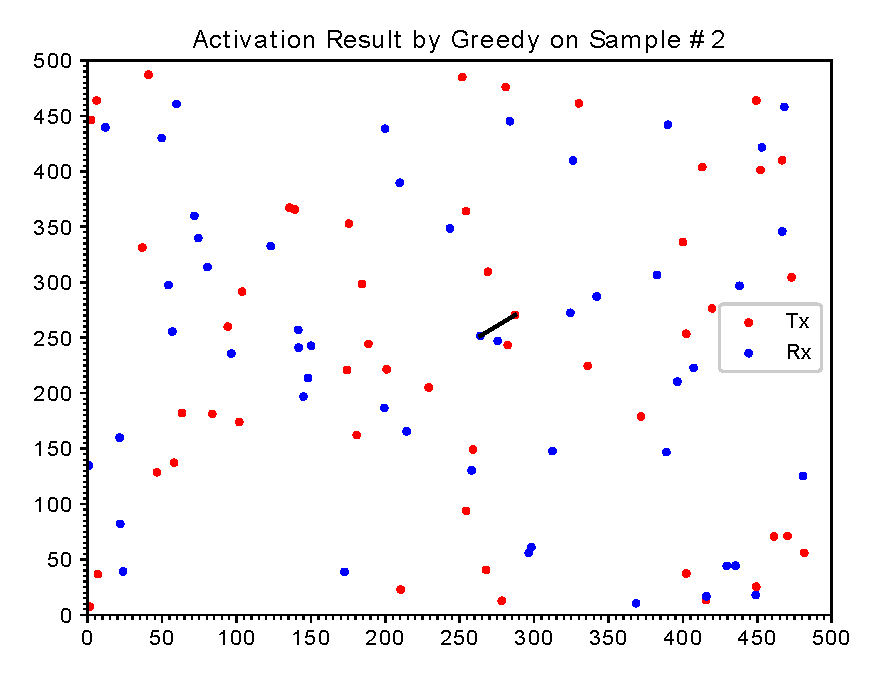
\includegraphics[width=8cm]{fig/premature_greedy}}
  \\
  \subfigure[FP]{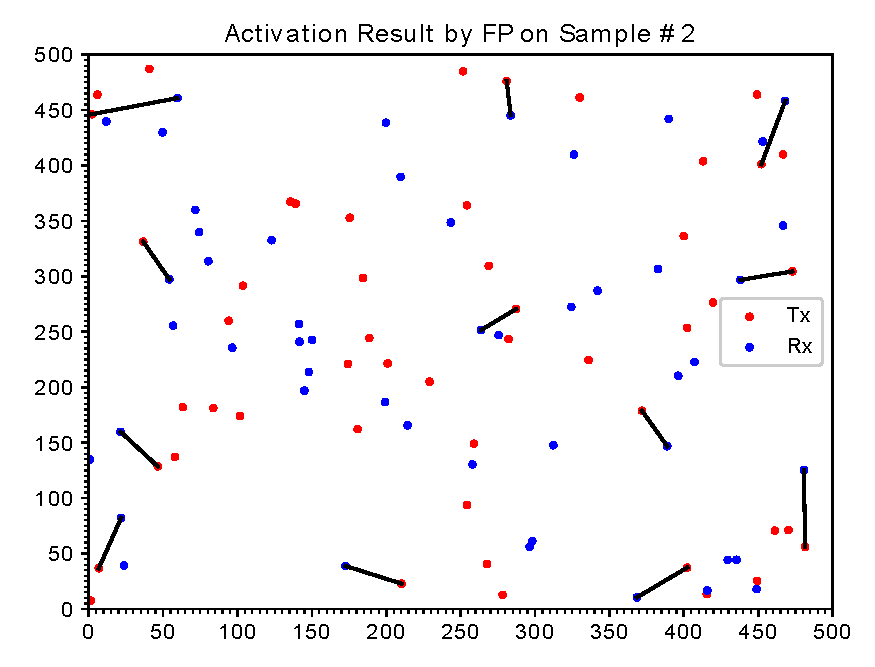
\includegraphics[width=7.5cm]{fig/premature_FP}}
  \subfigure[神经网络]{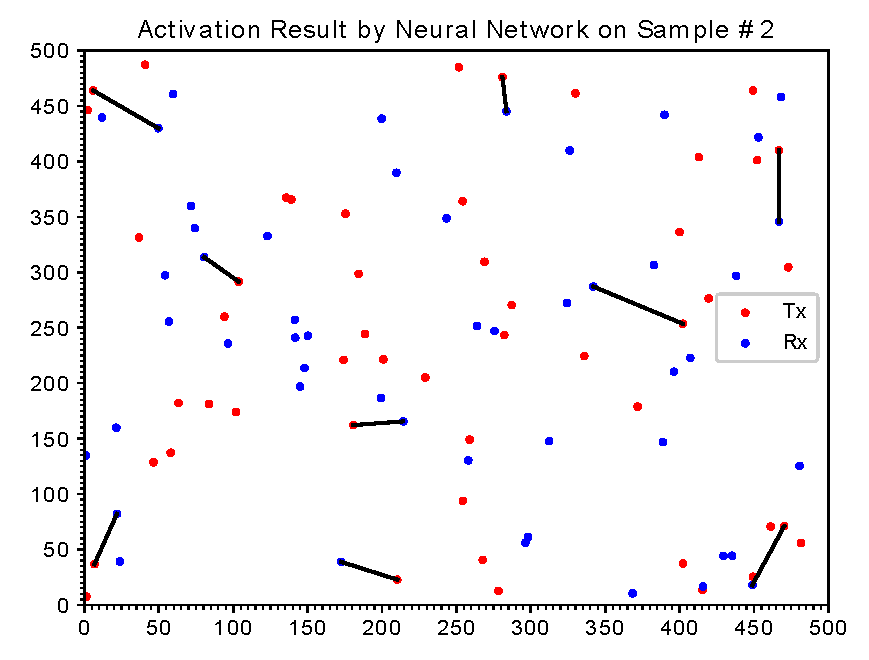
\includegraphics[width=7.5cm]{fig/premature_neuralnet}}
\caption{贪婪启发式方法过早激活最强链路}
\label{fig:greedyprematureproblem}
\end{figure}


如上述描述,在测试中,空间学习方法始终能够产生接近FPLinQ输出的调度模式,显示出神经网络能够学习到最先进的优化策略。在图\ref{fig:greedyprematureproblem}中展示的贪婪启发式方法示例中,该方法过早地激活了最强链路,导致了次优的调度决策。与之相反,神经网络能够更好地评估链路之间的相互影响和干扰,从而做出更有效的调度决策。

总体而言,这些测试结果表明,所提出的空间学习方法不仅能够在不需要显式知道信道信息的情况下实现接近最优调度的性能,而且还优于需要CSI的传统方法,如贪婪启发式方法。这为使用深度学习技术解决复杂的无线网络调度问题提供了一个有力的证明。

\subsection{在快速衰落下的总速率优化}

到目前为止,作者在仅具有路径损耗分量的信道上进行了测试(根据ITU-1411户外模型)。由于路径损耗由位置决定,信道本质上是位置的确定性函数。

在这一节中,作者将瑞利快速衰落引入到测试信道中。这更具挑战性,因为信道增益现在是地理位置信息(GLI)输入的随机函数。请注意,神经网络仍然使用不包含衰落的信道进行训练。

作者在500米乘500米的区域内使用50个D2D链路的测试布局,以及4种均匀链路距离分布。总速率性能结果如表\ref{tab:sumratesFastfading}所示,增加了一个额外的基准:
\begin{itemize}
\item {\bf 未考虑快速衰落的FP:} 基于没有快速衰落效应的CSI运行FP。这代表了在不知道快速衰落的情况下所能做到的最佳情况。
\end{itemize}

\begin{table}
\caption{在具有快速衰落信道上的总速率与FP百分比}
\centering
\begin{tabular}{|c|c||c|c|c|c|}
\hline
总速率 (\%) & CSI & 30m$\sim$70m & 2m$\sim$65m & 10m$\sim$50m & all 30m\\
\hline
空间深度学习 & \crossmark & 71.81 & 88.59 & 82.45 & 73.87 \\
\hline
未知快速衰落FP & \checkmark & 77.68 & 88.87 & 82.66 & 76.32 \\
\hline
贪婪 & \checkmark & 95.86 & 98.32 & 97.74 & 96.73 \\
\hline
最强链路 & \checkmark & 65.42 & 80.77 & 75.00 & 68.84 \\
\hline
随机 & \crossmark & 31.70 & 44.50 & 44.04 & 42.72 \\
\hline
全激活 & \crossmark & 25.28 & 50.42 & 43.82 & 38.38 \\
\hline
FP & \checkmark & 100 & 100 & 100 & 100 \\
\hline
\end{tabular}
\label{tab:sumratesFastfading}
\end{table}

如表\ref{tab:sumratesFastfading}所示,与FP或贪婪算法(这两者都需要精确CSI)相比,深度学习的性能确实显著下降。然而,鼓舞人心的是,神经网络的性能与\emph{未知快速衰落的FP}相匹配,表明它已经接近最优,考虑到只有GLI作为输入。

\subsection{计算复杂度}

在这一节中,作者进一步论证了所提出的神经网络与贪婪算法或FP算法相比在计算复杂度上具有优势,作者提供了理论分析和一些实验验证。

\subsubsection{理论分析}
作者首先提供每种方法的复杂度随链路数量$N$的比例函数:
\begin{itemize}
\item \textbf{FPLinQ算法}:
在每次迭代中,为了更新调度输出和相关量,主要计算包括与$N\times N$信道系数矩阵的矩阵乘法。因此,每次迭代的复杂度为$O(N^2)$。假设需要固定次数的迭代才能收敛,总运行时间复杂度为$O(N^2)$。
\item \textbf{贪婪启发式}:贪婪算法逐个链路顺序做出调度决策。在决定是否调度第$i$个链路时,它需要比较到目前为止已调度的所有链路的总速率,激活和不激活新链路的情况。这涉及重新计算干扰,计算量为$O(i)$。由于$i$从$1$到$N$变化,贪婪算法的总体复杂度因此为$O(N^2)$。
\item \textbf{神经网络} 假设离散化网格的维度为$K\times K$,空间滤波器的维度为$J\times J$。此外,设$h_0$为全连接阶段输入特征向量的大小,设$(h_1, h_2,...h_n)$为$n$个隐藏层的隐藏单元数目(注意输出层有一个单元)。所提出神经网络的总运行时间复杂度可以计算为:
\begin{align}
\underbrace{K^2 \times J^2}{\text{卷积阶段}} + N \times
\underbrace{(h_0h_1 + \dots + h{n-1}h_{n} + h_{n})}_{\text{每对全连接阶段}}
\end{align}
因此,在固定区域大小的布局下,神经网络的时间复杂度随$O(N)$比例增长。
\end{itemize}

\subsubsection{实验验证}
在实际实现中,由于能够利用并行计算架构,神经网络的运行时间甚至可以低于$O(N)$。为了说明这一点,作者测量了使用FP和贪婪算法以及使用所提出的神经网络调度不同数量D2D链路的布局的总计算时间。计时在单台桌面电脑上进行,硬件规格如下:
\begin{itemize}
\item FP和贪婪:英特尔CPU Core i7-8700K @ 3.70GHz
\item 神经网络:Nvidia GPU GeForce GTX 1080Ti
\end{itemize}
为了合理比较运行时间,作者选择最适合各算法的硬件。神经网络的实现高度可并行化;它极大地受益于GPU的并行计算能力。另一方面,FP和贪婪算法具有严格的顺序计算流程,因此更适合在CPU上运行,因为CPU的时钟速度要高得多。上述列出的CPU和GPU在其各自类别的计算能力和价格点上大致处于同一水平。

如图\ref{fig:varyDensityTime}所示,所提出的神经网络的计算复杂度大致是恒定的,并且确实比FP基线在具有大量D2D链路的布局中低几个数量级。

作者在此指出,复杂度比较本质上依赖于实现方式。例如,作者的神经网络实现的瓶颈是空间卷积,这是通过TensorFlow中的内置函数计算的\cite{tensorflow}。然而,TensorFlow中用于计算卷积的内置函数会在整个地理区域的每个位置进行卷积计算,这是过度的。如果使用定制的卷积算子只在特定的感兴趣位置进行计算,那么作者的神经网络的运行时间复杂度可以进一步降低。复杂度预计为$O(N)$,但常数要比图\ref{fig:varyDensityTime}中的复杂度曲线小得多。作者还要指出,传统优化方法的计算复杂度可以通过进一步的启发式方法来降低;例如,参见\cite{Guo_1000}。

\begin{figure}
\centering
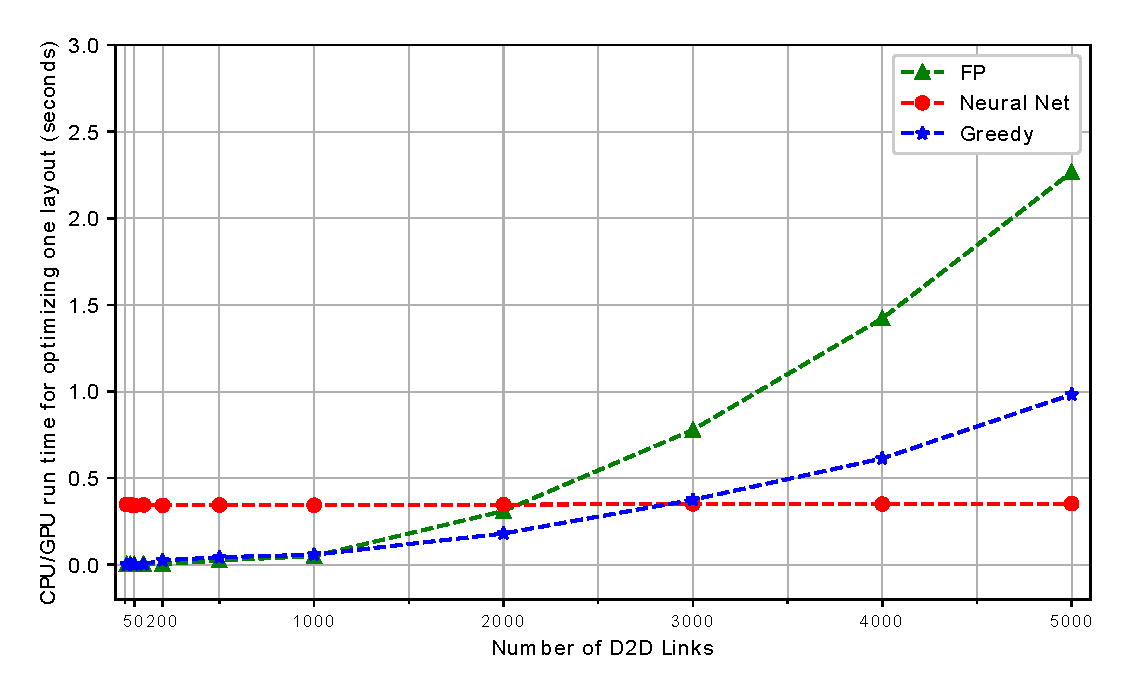
\includegraphics[width=11cm]{fig/VaryDensityTime}
\caption{具有不同数量D2D链路的布局的计算时间。}
\label{fig:varyDensityTime}
\end{figure}

总结来说,所提出的神经网络在大型网络中具有显著的计算复杂度优势,同时保持接近最优的调度性能。这一点非常值得注意,考虑到神经网络只在具有50个链路的布局上进行了训练,并且只需要$O(N)$的GLI而不是$O(N^2)$的CSI。

\clearpage

\section{该文章与本课程的关联性}

\subsection{瑞利衰落信道模型}


本课程在第二章提到的瑞利衰落(Rayleigh fading)是无线通信中描述非视距(Non-Line of Sight, NLOS)环境下信号传播的重要模型。这种衰落信道模型假设信号在通过无线信道后,其幅度呈随机变化,表现为衰落,且信号的包络服从瑞利分布(Rayleigh distribution)。瑞利衰落特别适用于描述由电离层和对流层反射的短波信道,以及建筑物密集的城市环境中的信号传播。在本文的算法测试中,作者引入了瑞利衰落以测试算法的鲁棒性。

在数学上,瑞利衰落的特性可以通过瑞利分布来描述。若随机变量 \( X \) 和 \( Y \) 独立且同分布,且均服从标准正态分布(均值为0,方差为 \(\sigma^2\)),则 \( Z = \sqrt{X^2 + Y^2} \) 服从瑞利分布。瑞利分布的概率密度函数(PDF)为 \( f(z; \sigma) = \frac{z}{\sigma^2} e^{-z^2 / (2\sigma^2)}, \quad z \geq 0 \),其中 \( \sigma \) 是信号幅度的标准差。这表明接收信号的功率级别是随机变化的,可以用信号包络的平方来表示。

瑞利衰落模型在无线通信系统中非常关键,尤其是在城市环境和没有直射路径的场景中。它对于设计和优化无线通信系统至关重要,特别是在考虑调制方案、功率控制、信道编码和信号处理策略等方面。多径效应导致的信号干扰和衰落可以表示为多个相互独立的信号分量的叠加,每个分量都有自己的振幅和相位,在瑞利衰落模型中,这些分量的振幅服从瑞利分布。

\subsection{MIMO}
本课程在第二章提到的MIMO(Multiple Input, Multiple Output)技术是无线通信中的一种关键技术,用于提高数据传输速率和通信系统的可靠性。MIMO通过在发送端(发射源)和接收端(接收器)都使用多个天线来工作。这些天线的组合有助于最小化错误、优化数据速度,并通过同时在多个信号路径上传输数据来提高无线传输的容量​​。

MIMO技术的一个重要应用是在LTE(Long-Term Evolution)和WiMAX(Worldwide Interoperability for Microwave Access)等无线宽带技术标准中的部署。LTE利用MIMO和OFDM(Orthogonal Frequency-Division Multiplexing,正交频分复用)提高速度,可达100 Mbps甚至更高。LTE使用MIMO进行发送多样性、空间复用(以传输空间分离的独立信道),以及单用户和多用户系统的支持。MIMO在LTE中不仅使数据传输更可靠,还提高了数据速率​​。

此外,MIMO技术也在5G系统中得到了进一步的发展和应用。所谓的“大规模5G MIMO系统”利用许多小天线增加用户带宽,不仅仅是传输速率,而且支持每个天线更多用户的连接。不同于4G MIMO使用的频分双工(FDD)系统,5G大规模MIMO使用了一种称为时分双工(TDD)的不同设置,这提供了相对于FDD的多种优势​​。

MIMO技术还包括了一种称为波束成形(Beamforming)的射频管理技术。在5G中,三维波束成形可以在用户的垂直和水平方向形成和指向信号束。这些信号束甚至可以到达高层建筑的顶部的设备,防止与其他无线信号的干扰,并随着用户在特定区域内移动而保持连接​​。

这篇文章中的技术主要可以影响空间复用、干扰管理以及网络容量和吞吐量方面。该研究利用深度学习进行无线网络调度优化,特别是频谱优化和资源分配,这与MIMO的空间复用技术密切相关,有助于提高数据传输速率。同时,深度学习在处理信号干扰方面的应用对于MIMO系统中的干扰管理也极为重要。此外,优化算法还可提升MIMO系统的网络容量和总体吞吐量,进而提高网络性能。
\clearpage
\section{文章的重点和难点}
\subsection{文章重点}

本篇论文的核心目标是探究如何在全频率复用的密集无线网络中最优化地调度干扰链路。关键的研究贡献和发现如下:

\begin{enumerate}
  \item \textbf{深度学习模型的提议:} 提出了一种新的基于地理位置信息的深度学习架构,用于快速有效地调度干扰链路,避免了传统方法中昂贵的信道估计过程。
   
  \item \textbf{地理空间卷积:} 研究开发了一种新颖的神经网络架构,能够通过对传输节点和接收节点的地理位置进行空间卷积,来估算节点间的干扰情况。公式化为:
   \[
   \text{Conv}(X, W) = W * X
   \]
   其中\(X\)代表地理位置信息矩阵,\(W\)代表卷积核,\(*\)是卷积运算。

  \item \textbf{迭代反馈结构:} 通过包括反馈连接的迭代优化过程,神经网络不断调整链路的激活状态,在不断迭代中逼近最优调度方案。

  \item \textbf{无监督学习机制:} 采用无监督方法训练神经网络,以在不直接知道链路之间干扰情况的前提下学习调度策略。优化目标为总和速率,调度问题的表达可以建模为一个离散优化问题,形式化为:
 
  \[\max_{\mathbf{s}} U(\mathbf{s}) = \sum_{i=1}^{N} w_i \cdot \log(1+\text{SINR}_i(\mathbf{s}))\]
  
  其中,\( \mathbf{s} \)表示链路的调度向量,\( \text{SINR}_i \)是第\( i \)个链路的信噪比,\( w_i \)为链路\( i \)的权重,通常用于实现比例公平性。

  \item \textbf{调度策略的泛化能力:} 神经网络在学习后拥有泛化到更大规模网络以及不同链路密度网络的能力,证明了该方法的扩展性。
\end{enumerate}

\subsection{文章难点}

如何在深度学习中结合地理位置信息来准确和高效地进行无线链路调度,是论文中的核心挑战。主要难点包括:

\begin{enumerate}
  \item \textbf{无监督学习优化目标的设计:} 设计一个合适的学习目标,使得无监督神经网络可以自动学习到最优调度策略,并且保证在实际无线网络中该目标仍然有效。

  \item \textbf{神经网络架构设计:}设计一个深度神经网络结构,能够高效处理和提取地理空间信息,并在之上构建反馈和卷积机制,实现空间信息的有效学习。

  \item \textbf{空间卷积的执行:}实现和优化地理空间卷积操作,使其能够准确估计链路之间基于地理位置的潜在干扰,对于大规模数据的处理提出了高效的空间卷积算法。

  \item \textbf{调度算法的泛化性:} 面临在不同网络大小和链路密度条件下神经网络性能的泛化问题。如何保证一个网络模型能够在多种不同的网络设置中获得满意的性能。

  \item \textbf{学习过程与收敛性:} 在引入瑞利快速衰落的情况下,信道增益成为GLI输入的随机函数,保证神经网络能够学习到有效的链路调度策略,并保证训练过程的稳定收敛。
  
  \item \textbf{计算资源与运行时间:} 虽然神经网络可以减少传统调度算法的计算复杂度,但依旧需要处理大型网络模型的训练,和高效利用计算资源。
  
  \item \textbf{性能评估与验证:}评估深度学习方法与现有算法比如贪婪算法和信道感知的调度算法的性能比较,并验证在实际网络环境中的有效性。
  \end{enumerate}

\clearpage
  \section{不足和改进方向}

  \subsection{快速衰落环境的适应性:}
  \begin{itemize}
      \item \textbf{当前状态:} 在引入瑞利快速衰落的情况下,神经网络的性能相比于需要精确CSI的传统方法有所下降。
      \item \textbf{改进方向:} 可以考虑在神经网络训练过程中加入模拟快速衰落的信道模型,例如:
      \[
      h = h_{\text{path-loss}} \cdot h_{\text{Rayleigh}}
      \]
      其中,\( h_{\text{path-loss}} \) 表示路径损耗成分,\( h_{\text{Rayleigh}} \) 代表瑞利衰落成分。
  \end{itemize}
  
  \subsection{计算复杂度优化:}
  \begin{itemize}
      \item \textbf{当前状态:} 尽管神经网络在大型网络中的计算复杂度优势显著,但空间卷积的计算效率可能成为瓶颈。
      \item \textbf{改进方向:} 优化空间卷积的实现。可将卷积阶段的复杂度从当前的\( O(K^2 \times J^2) \)降低到与激活链路数量成比例的\( O(N \times J^2) \)。
  \end{itemize}
  
  \subsection{模型泛化和训练策略:}
  \begin{itemize}
      \item \textbf{当前状态:} 神经网络表现出对不同链路密度布局的泛化能力。
      \item \textbf{改进方向:} 
          \begin{itemize}
              \item 使用更多样化的数据集。
              \item 探索多任务学习策略。
              \item 进行迁移学习的微调。
          \end{itemize}
  \end{itemize}
  
  

\bibliographystyle{IEEEtran}
\bibliography{learning}
\end{document}